\documentclass[12pt]{ctexart}
\usepackage{geometry}       % 设置页面整体布局
\geometry{top=2.5cm, bottom=2.5cm, left=2cm, right=2cm}
\usepackage{fancyhdr}       % 设置页眉页脚布局
\pagestyle{fancy}
\rhead{\thepage}            % 设置右页眉为页数
\chead{中国科学技术大学}
\cfoot{}                    % 设置中间页脚为空
\usepackage{amsmath}        % 数学公式宏包
\numberwithin{equation}{section}
\usepackage{esint}          % 交叉引用宏包
\usepackage[colorlinks,     % 设置引用的颜色
            linkcolor=black,
            anchorcolor=black,
            urlcolor=cyan,
            citecolor=black,
           ]{hyperref}
\usepackage{makecell}       % 插入表格宏包
\usepackage{longtable}      % 长表格宏包
\usepackage{appendix}       % 生成附录宏包
\usepackage{graphicx}       % 插入图片宏包
\usepackage{epstopdf}       % 插入eps图片宏包
\usepackage{cite}           % 文献引用宏包
\renewcommand{\thefigure}   % 设置图片编号格式
    {\thesection{}.\arabic{figure}}
\renewcommand{\thefootnote}{} % 设置角标编号不出现在文中
                            % 以\footnotetext{Footnotetext without footnote mark}使用
\usepackage{unicode-math}
\usepackage{listings}
\usepackage{hyperref}



\CTEXsetup[format={\Large\bfseries}]{section}


\begin{document}

\nocite{*}

\begin{center}
    \heiti \fontsize{24pt}{0}{正丁醇偶极矩的测定}

    \vspace{12pt}

    \kaishu \fontsize{13.75pt}{0}禤科材

    \footnotetext{\textbf{实验日期:}2022年11月11日}
    \footnotetext{\textbf{作者简介:}禤科材(2002-),男,学号PB20030874,中国科学技术大学本科在读,专业方向为化学物理}
    \footnotetext{\textbf{联系方式:}电话 18108064415 ,邮箱 \href{mailto:ustcxkc@mail.ustc.edu.cn}{ustcxkc@mail.ustc.edu.cn}}

    \vspace{5pt}

    \songti \fontsize{12pt}{0}(中国科学技术大学化学与材料科学学院,安徽 合肥 230026)
\end{center}

\noindent\textbf{摘~~~\!要}~~~\!
分子的极性可以体现在诸如物质的介电常数,折射率等可测量的物理量上。
通过测定这些物理量我们可以测定极性分子的偶极矩大小。本实验根据
Clausius-Mosotti-Debye 方程,通过测定不同浓度下正丁醇—环己烷
溶液的密度,折射率,介电常数等物理量外推出无限稀释下的摩尔折射率和
摩尔极化率,从而计算出正丁醇分子的偶极矩。
\newline
\textbf{关键字}~~~\!
正丁醇;偶极矩;摩尔折射度;摩尔极化度

\begin{center}
    {\LARGE\rmfamily\textbf{Determination of the Dipole Moment of n-Butanol}}

    \vspace{12pt}

    {\slshape Xuan Kecai}

    \vspace{5pt}

    (School of Chemistry and Material Science, USTC, Hefei 230026, China)
\end{center}

\noindent\textbf{Abstract}~~~\!
The polarity of a molecule can be reflected in measurable
physical quantities such as the dielectric constant and
refractive index of the substance. By measuring these
physical quantities, we can determine the dipole moment of
polar molecules. According to the Clausius-Mosotti-Debye
equation, this experiment extrapolates the molar refractive
index and molar polarizability under infinite dilution by
measuring the density, refractive index, and dielectric
constant of the n-butanol-cyclohexane solution at different
concentrations. Calculate the dipole moment of the n-butanol
molecule.
\newline
\textbf{Keywords}~~~\!
n-butanol; dipole moment; molar refractive index;
molar polarization

\section{序言}

由于空间构型的不同,分子的正负电荷中心可能重合,也可能不重合,其中
前者称为非极性分子,后者称为极性分子。$^{[1]}$分子的极性可用偶极矩
来表示,两个大小相等符号相反的电荷系统的电偶极矩为
\begin{align}
    \vec{\mu} = q\vec{r}.
\end{align}
其中$\vec{r}$是两个电荷中心间距矢量,方向是从正电荷指向负电荷,$q$
为电荷量,$\vec{\mu}$的单位为 Debye。对于偶极矩有 Clausius-
Mosotti-Debye 方程
\begin{align}
    \frac{\varepsilon-1}{\varepsilon+2}\cdot\frac{M}{\rho}
    = \frac{4\pi N_0}{3}
    \left(\alpha_E + \alpha_A + \frac{\mu^2}{3k_BT}\right).
\end{align}
其中$\mu$为极性分子的永久偶极矩,$k_B$为玻尔兹曼常数,$T$为开尔文
温度。

对于由溶剂 1 和溶剂 2 组成的溶液体系,根据 Hedestrand 理论,其
介电常数、折射率、摩尔极化度以及密度均和浓度成线性关系,即
\begin{align}
    \varepsilon &= \varepsilon_1(1+\alpha X_2), \\
    n &= n_1(1+\gamma X_2), \\
    \rho &= \rho_1(1+\beta X_2), \\
    P &= X_1P_1 + X_2P_2.
\end{align}

无限稀释的摩尔极化度$P^\infty$和无限稀释的摩尔折射度$R^\infty$
可由下式计算
\begin{align}
    P^\infty &= \frac{3\alpha\varepsilon_1}
            {(\varepsilon_1 + 2)^2}\cdot\frac{M_1}{\rho_1}
        + \frac{\varepsilon_1 - 1}{\varepsilon_1 + 2}\cdot
            \frac{M_2 - \beta M_1}{\rho_1}, \\
    R^\infty &= \frac{n_1^2 - 1}{n_1^2 + 2}\cdot
            \frac{M_2 - \beta M_1}{\rho_1}
        + \frac{6n_1^2 M_1 \gamma}{(n_1^2 + 2)^2\rho_1}.
\end{align}

故分子的永久偶极矩$\mu$为
\begin{align}
    \mu = 0.0128\sqrt{(P^\infty - R^\infty)T}.
\end{align}

\section{实验}
\subsection{试剂与仪器}

乙醇(无水乙醇)(国药集团化学试剂有限公司,AR)、环己烷(国药集团
化学试剂有限公司,AR)、正丁醇(硫酸亚铁铵)(国药集团化学试剂有限
公司,AR)、蒸馏水。

DMA 4100M 型密度计(Anton Paar)、KCP PLUS-B08W 型蠕动泵
(Kamoer)、HK-2A 型超级恒温水水浴(南京南大万和科技有限公司)、
PCM-1A 型介电常数测量仪(南京南大万和科技有限公司)、CP3235 型
分析天平(sartorius)、Abbemat 300 型自动折光仪(Anton Paar)、
吹风机、25mL 容量瓶、10mL 量筒、胶头滴管、烧杯。

\subsection{实验方法}
\subsubsection{折射率的测定}

配制摩尔分数分别为0\%、1\%、5\%、10\% 和15\% 的环已烷溶液各 25mL,
用阿贝折射仪测量三次溶液的折射率,取平均值。

\subsubsection{介电常数的测定}

已知真空下的电容$C_o = 3.96$PF,向电容池中从低到高依次注入不同
浓度的溶液使液面没过探头,测定不同浓度的电容。每次更换溶液时使用
吹风机将全部易挥发的溶液吹干。

\subsubsection{溶液密度的测定}

用蠕动泵向密度计中送入溶液,记录温度稳定的密度度数。

\section{结果与讨论}
\subsection{实验结果}

\begin{longtable}{c|ccccc}
    \caption{实验结果} \\
    \hline
    实验样品序号 & 1 & 2 & 3 & 4 & 5 \\
    \hline
    溶剂摩尔分数$X_1$ & 100. &  97.12 &  95.66 &  90.75 &  86.58  \\
    \hline
    溶质摩尔分数$X_2$ & 0. &  2.87 &  4.33 &  9.24 &  13.41  \\
    \hline
    电容平均值/PF & 6.52 & 6.68 & 6.76 & 7.06 & 7.42 \\
    \hline
    电容校正值/PF & 2.55 & 2.73 & 2.79 & 3.17 & 3.54 \\
    \hline
    折光率均值/nD & 1.4209 & 1.4196 & 1.4190 & 1.4171 & 1.4159 \\
    \hline
    密度/(g$\cdot$cm$^{-3}$) & 0.7691 & 0.7692 & 0.7694 & 0.7703 & 0.7711 \\
    \hline
\end{longtable}

表 1 为 30.00$^\circ$C 条件下不同浓度溶液的数据测量结果。经计算得到
\begin{align}
    \alpha &= 1.308, \\
    \beta &= 0.1908, \\
    \gamma &= -0.0227.
\end{align}

带入式(1.7)、(1.8)得到
\begin{align}
    P^\infty &= 78.09 ~\mathrm{cm^3\cdot mol^{-1}}, \\
    R^\infty &= 17.28 ~\mathrm{cm^3\cdot mol^{-1}}.
\end{align}

再带入式(1.9)可以计算出正丁醇分子的偶极矩为 1.74 Debye。

由高斯软件 $^{[2]}$ 计算得到不同状态下的偶极矩和单点能结果,
导出数据如表 2 所示。

\begin{longtable}{ccccccc}
    \caption{不同参数及方法下的偶极矩与单点能计算结果} \\
    \hline
    序号 & 计算方法 & 基组 & 状态 & 任务类型 & 偶极矩(Debye)
        & 单点能(A.U.) \\
    \hline
     1 & DFT/B3LYP &   3-21+g*    & 环己烷溶液 & 结构优化 & 2.3852 & / \\
     2 & DFT/B3LYP & 6-31+g(d,p)  & 环己烷溶液 & 能量计算 & 2.0057 & -233.69 \\
     3 & DFT/B3LYP & 6-311+g(d,p) & 环己烷溶液 & 能量计算 & 1.9900 & -233.74 \\
     4 & DFT/B3LYP & aug-cc-pvdz  & 环己烷溶液 & 能量计算 & 1.8265 & -233.70 \\
     5 &    MP2    & 6-311+g(d,p) & 环己烷溶液 & 能量计算 & 2.1430 & -232.21 \\
     6 & DFT/B3LYP &   3-21+g*    &    气相   & 结构优化 & 2.1903 & / \\
     7 & DFT/B3LYP & 6-31+g(d,p)  &    气相   & 能量计算 & 1.8167 & -233.69 \\
     8 & DFT/B3LYP & 6-311+g(d,p) &    气相   & 能量计算 & 1.7995 & -233.74 \\
     9 & DFT/B3LYP & aug-cc-pvdz  &    气相   & 能量计算 & 1.6387 & -233.70 \\
    10 &    MP2    & 6-311+g(d,p) &    气相   & 能量计算 & 1.9508 & -232.21 \\
    \hline
\end{longtable}

所有计算均收敛。

\subsection{误差分析}
\subsubsection{系统误差}

(1)溶液法测得的溶质偶极矩与气相测得的真实值存在一定的偏差。造成
这种现象的原因是非极性溶剂与极性溶质分子相互间的作用,即溶剂化作用。
这种偏差现象溶剂效应。可使用理论方法对此误差进行校正,如将溶剂化
作用考虑为外部势场,计算正丁醇分子在此势场中的偶极矩,即可进行校正。

(2)公式推导中认为原子极化度只有电子极化度的$5\%\sim 10\%$,故
忽略了原子极化度。但准确的测量需要考虑原子极化度的影响,忽略其影响
会导致实验结果偏大。同时实验原理还忽略了正丁醇分子间的相互作用项,
因而采用外推法得到无限稀释条件下的$P^\infty$、$R^\infty$,但无限
稀释的状态只能是假想的状态,实际并不存在,这导致实验结果与实际结果
存在一定的偏差。

\subsubsection{偶然误差}

(1)本实验所使用的环己烷是易挥发的有机物,而正丁醇在室温下挥发
较少。溶剂的挥发会导致溶液浓度发生变化,从而给最终的实验结果带来
一定的误差。因此在实验中溶液配好后应迅速盖上瓶盖,实验中取用溶液等
操作也要迅速进行,以减少挥发。

(2)本实验所测量的物理量密度,折光率,介电常数均与温度有关,所以
全程需要有恒温装置对样品进行恒温处理。安东帕折射仪与密度测量仪结构
较为精密,其温度能够被较好的控制。而电容测定时实验温度由恒温水浴锅
及循环水进行控制。循环水在橡胶管中流一段时间后温度会下降,到达
电容池时温度会低于所需控制的30$^\circ$C。这一温差变化会给实验结果
带来一定程度的误差。

(3)实验测量电容时,电容池内液体难以被完全吹干。且即使液体被吹干,
电容池附近的空气中仍含有大量的环己烷和正丁醇。这一现象会导致电容池
中的溶液浓度发生微小的改变,从而给实验结果带来一定的误差。

\subsection{实验体会与认识}

\subsubsection{实验结果讨论}

由高斯程序的计算结果(表 2)可以看出,不同方法计算得到的单点能的值
均在-232.7 a.u. 左右,相差无几,且迭代计算均收敛,这说明计算结果
是可信的。对比可知,环己烷的溶剂化效应会使正丁醇分子的偶极矩升高,
大约升高 0.2 Debye。还可以看出,选用不同方法、不同基组进行计算
会给计算结果带来一定的影响。用 MP2 计算得到的单点能比用 DFT 方法
计算得到的结果绝对值略小;选用更大的基组计算得到的偶极矩的值会更小。

将实验与计算结果进行对比可以看出,实验得到的偶极矩的值为 1.74
Debye,这与用 DFT / B3LYP 方法在 aug-cc-pvdz 基组下计算的
偶极矩的值相一致,而比其他方法计算的值偏小。考虑到 aug-cc-pvdz
基组较大,弥散函数较多,计算结果应当更加准确。

计算结果指出,气相中环己烷分子的偶极矩比液相中的小约 0.2 Debye。
特别的,对于用 DFT / B3LYP 方法在 aug-cc-pvdz 基组下计算得到的
结果,溶剂化效应的修正量为 0.1878 Debye。考虑这一溶剂化因素的修正,
实验得到的正丁醇分子的偶极矩值应被修正为 1.55 Debye。查阅资料
得到正丁醇分子的偶极矩为 1.66 Debye $^{[3]}$,可见实验值与真实值
符合较好。

\section{结语}

本实验通过测量不同浓度正丁醇的环己烷溶液的折光率、密度、介电常数
计算出了正丁醇的偶极矩为 1.74 Debye,若考虑溶剂化因素的理论修正,
则偶极矩应为 1.55 Debye,这与理论值符合较好。

\begin{center}
    \Large\bfseries{参考文献}
\end{center}
\noindent
[1] 张祖德. 无机化学. 修订版[M]. 中国科学技术大学出版社, 2010.

\noindent
[2] GaussView, Version 6, Dennington, Roy; Keith, Todd A.;
Millam, John M. Semichem Inc., Shawnee Mission, KS, 2016.

\noindent
[3] J.A. 迪安, 迪安, Dean, et al. 兰氏化学手册 [M]. 科学出版社,
2003.

\newpage

\begin{center}
    \LARGE\bfseries{附录~~~实验数据处理}
\end{center}
\begin{center}
    \Large\bfseries{附录I~~~实验数据处理}
\end{center}

空气电容值的平均值为 4.11 PF。

实验测量数据的处理结果如下表所示。
\begin{longtable}{c|ccccc}
    \caption{实验数据处理} \\
    \hline
    实验样品序号 & 1 & 2 & 3 & 4 & 5 \\
    \hline
    环己烷质量/g & 15.282 &  15.632 &  15.505 &  14.296 &  14.813  \\
    \hline
    环己烷物质的量/mol & 0.1816 & 0.1857 & 0.1842 & 0.1698 & 0.1760 \\
    \hline
    正丁醇质量/g & 0.000 &  0.463 &  0.702 &  1.456 &  2.296  \\
    \hline
    正丁醇物质的量/mol & 0.000 & 0.00694 & 0.00911 & 0.0208 & 0.0307 \\
    \hline
    溶剂摩尔分数$X_1$/\% & 100. &  97.12 &  95.66 &  90.75 &  86.58  \\
    \hline
    溶质摩尔分数$X_2$/\% & 0. &  2.87 &  4.33 &  9.24 &  13.41  \\
    \hline
    电容平均值/PF & 6.52 & 6.68 & 6.76 & 7.06 & 7.42 \\
    \hline
    电容校正值/PF & 2.55 & 2.73 & 2.79 & 3.17 & 3.54 \\
    \hline
    折光率均值/nD & 1.4209 & 1.4196 & 1.4190 & 1.4171 & 1.4159 \\
    \hline
    密度/(g$\cdot$cm$^{-3}$) & 0.7691 & 0.7692 & 0.7694 & 0.7703 & 0.7711 \\
    \hline
\end{longtable}

\subsection*{I.1~~~$\beta$的计算}

作$\rho\sim X_2$线性拟合,拟合方程为
\begin{align}
    \rho = 0.01467 X_2 + 0.7689.
    \tag{I.1}
\end{align}

$\rho\sim X_2$拟合直线如图 4.1 所示。
\begin{figure}[!h]
    \centering
    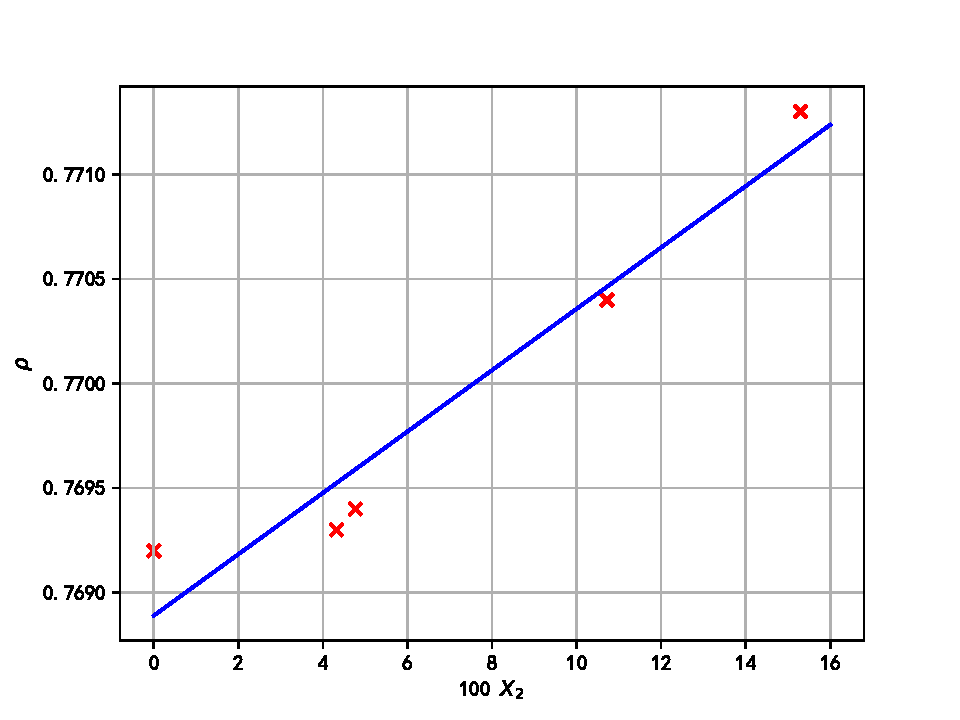
\includegraphics[scale=0.7]{fitting_beta.pdf}
    \caption{$\rho\sim X_2$拟合直线}
\end{figure}

对比(1.5)式可得
\begin{align}
    \beta = \frac{0.01467}{0.7689} = 0.1908.
    \tag{I.2}
\end{align}

\subsection*{I.2~~~$\gamma$的计算}

作$n \sim X_2$线性拟合,拟合方程为
\begin{align}
    n = -0.0322 X_2 + 1.421.
    \tag{I.3}
\end{align}

$n \sim X_2$拟合直线如图 4.2 所示。
\begin{figure}[!h]
    \centering
    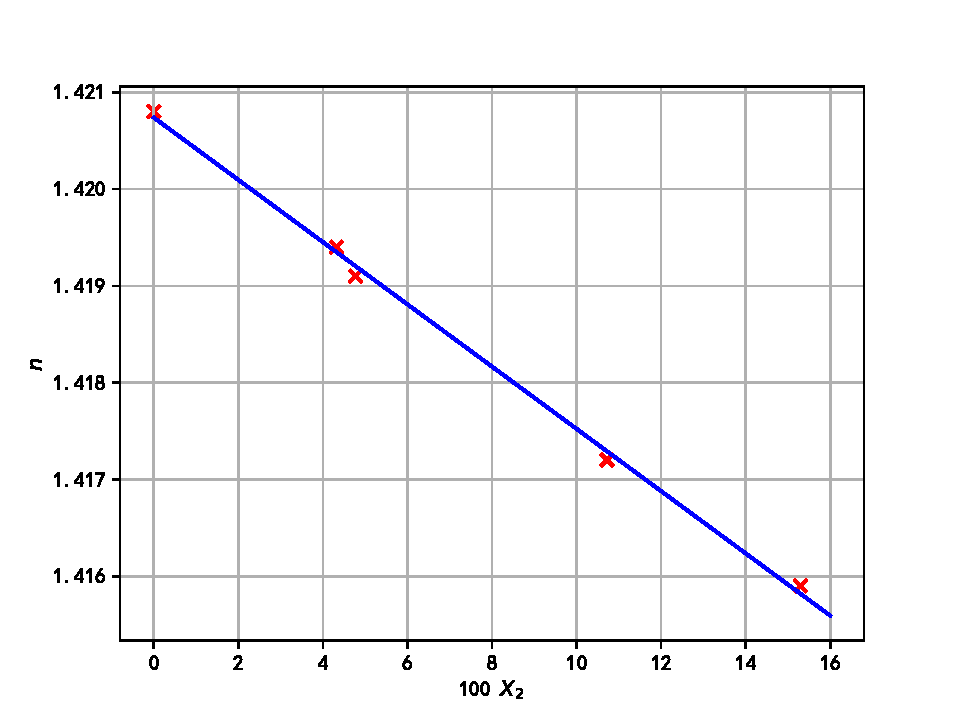
\includegraphics[scale=0.7]{fitting_gamma.pdf}
    \caption{$n \sim X_2$拟合直线}
\end{figure}

对比(1.4)式可得
\begin{align}
    \gamma = \frac{-0.0322}{1.421} = -0.0227.
    \tag{I.4}
\end{align}

\subsection*{I.3~~~$\alpha$的计算}

已知本实验条件下的电容有以下关系
\begin{align}
    \varepsilon_\text{环} &= \frac{C_\text{环}}{C_0}
        = 2.023 - 0.0016(t - 20), \tag{I.5} \\
    C'_\text{环} &= C_\text{环} + C_d, \tag{I.6} \\
    C'_0 &= C_0 + C_d, \tag{I.7} \\
    \varepsilon_\text{环}
        &= \frac{C'_\text{环}-C_d}{C'_0 - C_d}
        = 2.007. \tag{I.8}
\end{align}

已知$C'_0 = 3.69$ PF,$C'_\text{环} = 6.24$ PF,带入解得
$C_d = 1.158$ PF,因此$C_0 = 2.532$ PF。

故$\varepsilon = (C_\text{测} - C_d)/C_0$。
作$\varepsilon\sim X_2$线性拟合,拟合方程为
\begin{align}
    \varepsilon = 2.597 X_2 + 1.985. \tag{I.9}
\end{align}

$\varepsilon\sim X_2$拟合直线如图 4.3 所示。
\begin{figure}[!h]
    \centering
    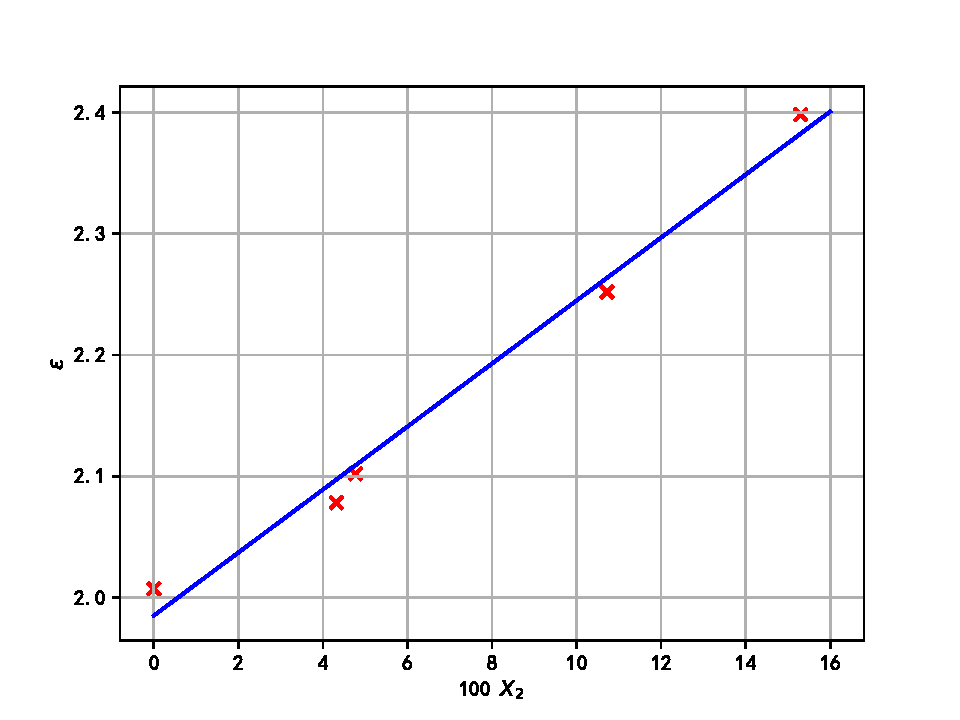
\includegraphics[scale=0.7]{fitting_alpha.pdf}
    \caption{$\varepsilon\sim X_2$拟合直线}
\end{figure}

对比(1.3)式可得
\begin{align}
    \alpha = \frac{2.597}{1.985} = 1.308.
    \tag{I.10}
\end{align}

\subsection*{I.4~~~$P^{\infty}$和$R^{\infty}$的计算}

摩尔极化度$P^\infty$和摩尔折射度$R^\infty$分别满足式(1.7)和
式(1.8)。代入数据即可算出
\begin{align}
    P^\infty
    &= \frac{3\alpha\varepsilon_1}{(\varepsilon_1 + 2)^2}
        \cdot\frac{M_1}{\rho_1}
        + \frac{\varepsilon_1 - 1}{\varepsilon_1 + 2}
        \cdot\frac{M_2 - \beta M_1}{\rho_1} \notag \\
    &= \frac{3\times 1.308\times 2.494}{(2.494+2)^2}
        \times \frac{84.096}{0.7689} + \frac{2.494-1}{2.494+2}
        \times \frac{74.08-0.1908\times 84.096}{0.7689} \notag \\
    &= 78.09 ~\mathrm{(cm^3\cdot mol^{-1})}, \tag{I.11} \\
    R^\infty
    &= \frac{n_1^2 - 1}{n_1^2 + 2}
        \cdot\frac{M_2 - \beta M_1}{\rho_1}
        + \frac{6n_1^2 M_1 \gamma}{(n_1^2 + 2)^2\rho_1} \notag \\
    &= \frac{1.421^2-1}{1.421^2+2}
        \times \frac{74.08-0.1908\times 84.096}{0.7689}
        + \frac{6\times 1.421^2\times 84.096\times (-0.0227)}
               {(1.421^2+2)^2\times 0.7689} \notag \\
    &= 17.28 ~\mathrm{(cm^3\cdot mol^{-1})}. \tag{I.12}
\end{align}

\subsection*{I.5~~~$\mu$的计算}

正丁醇的偶极矩满足式(1.9)。代入数据即可算出
\begin{align}
    \mu
    &= 0.0128\sqrt{(P^\infty - R^\infty)T} \notag \\
    &= 0.0128\times\sqrt{(78.09-17.28)\times 303.15} \notag \\
    &= 1.74 ~\mathrm{(Debye)}. \tag{I.13}
\end{align}

故实验得到正丁醇分子的偶极矩为 1.74 Debye。

\newpage
\begin{center}
    \Large\bfseries{附录II~~~原始数据记录}
\end{center}

高斯程序计算导出结果如下表所示。

\begin{longtable}{ccccccc}
    \caption{不同参数及方法下的偶极矩与单点能计算结果} \\
    \hline
    序号 & 计算方法 & 基组 & 状态 & 任务类型 & 偶极矩(Debye)
        & 单点能(A.U.) \\
    \hline
     1 & DFT/B3LYP &   3-21+g*    & 环己烷溶液 & 结构优化 & 2.3852 & / \\
     2 & DFT/B3LYP & 6-31+g(d,p)  & 环己烷溶液 & 能量计算 & 2.0057 & -233.69 \\
     3 & DFT/B3LYP & 6-311+g(d,p) & 环己烷溶液 & 能量计算 & 1.9900 & -233.74 \\
     4 & DFT/B3LYP & aug-cc-pvdz  & 环己烷溶液 & 能量计算 & 1.8265 & -233.70 \\
     5 &    MP2    & 6-311+g(d,p) & 环己烷溶液 & 能量计算 & 2.1430 & -232.21 \\
     6 & DFT/B3LYP &   3-21+g*    &    气相   & 结构优化 & 2.1903 & / \\
     7 & DFT/B3LYP & 6-31+g(d,p)  &    气相   & 能量计算 & 1.8167 & -233.69 \\
     8 & DFT/B3LYP & 6-311+g(d,p) &    气相   & 能量计算 & 1.7995 & -233.74 \\
     9 & DFT/B3LYP & aug-cc-pvdz  &    气相   & 能量计算 & 1.6387 & -233.70 \\
    10 &    MP2    & 6-311+g(d,p) &    气相   & 能量计算 & 1.9508 & -232.21 \\
    \hline
\end{longtable}

\pagebreak

\begin{figure}[ht]
    \centering
    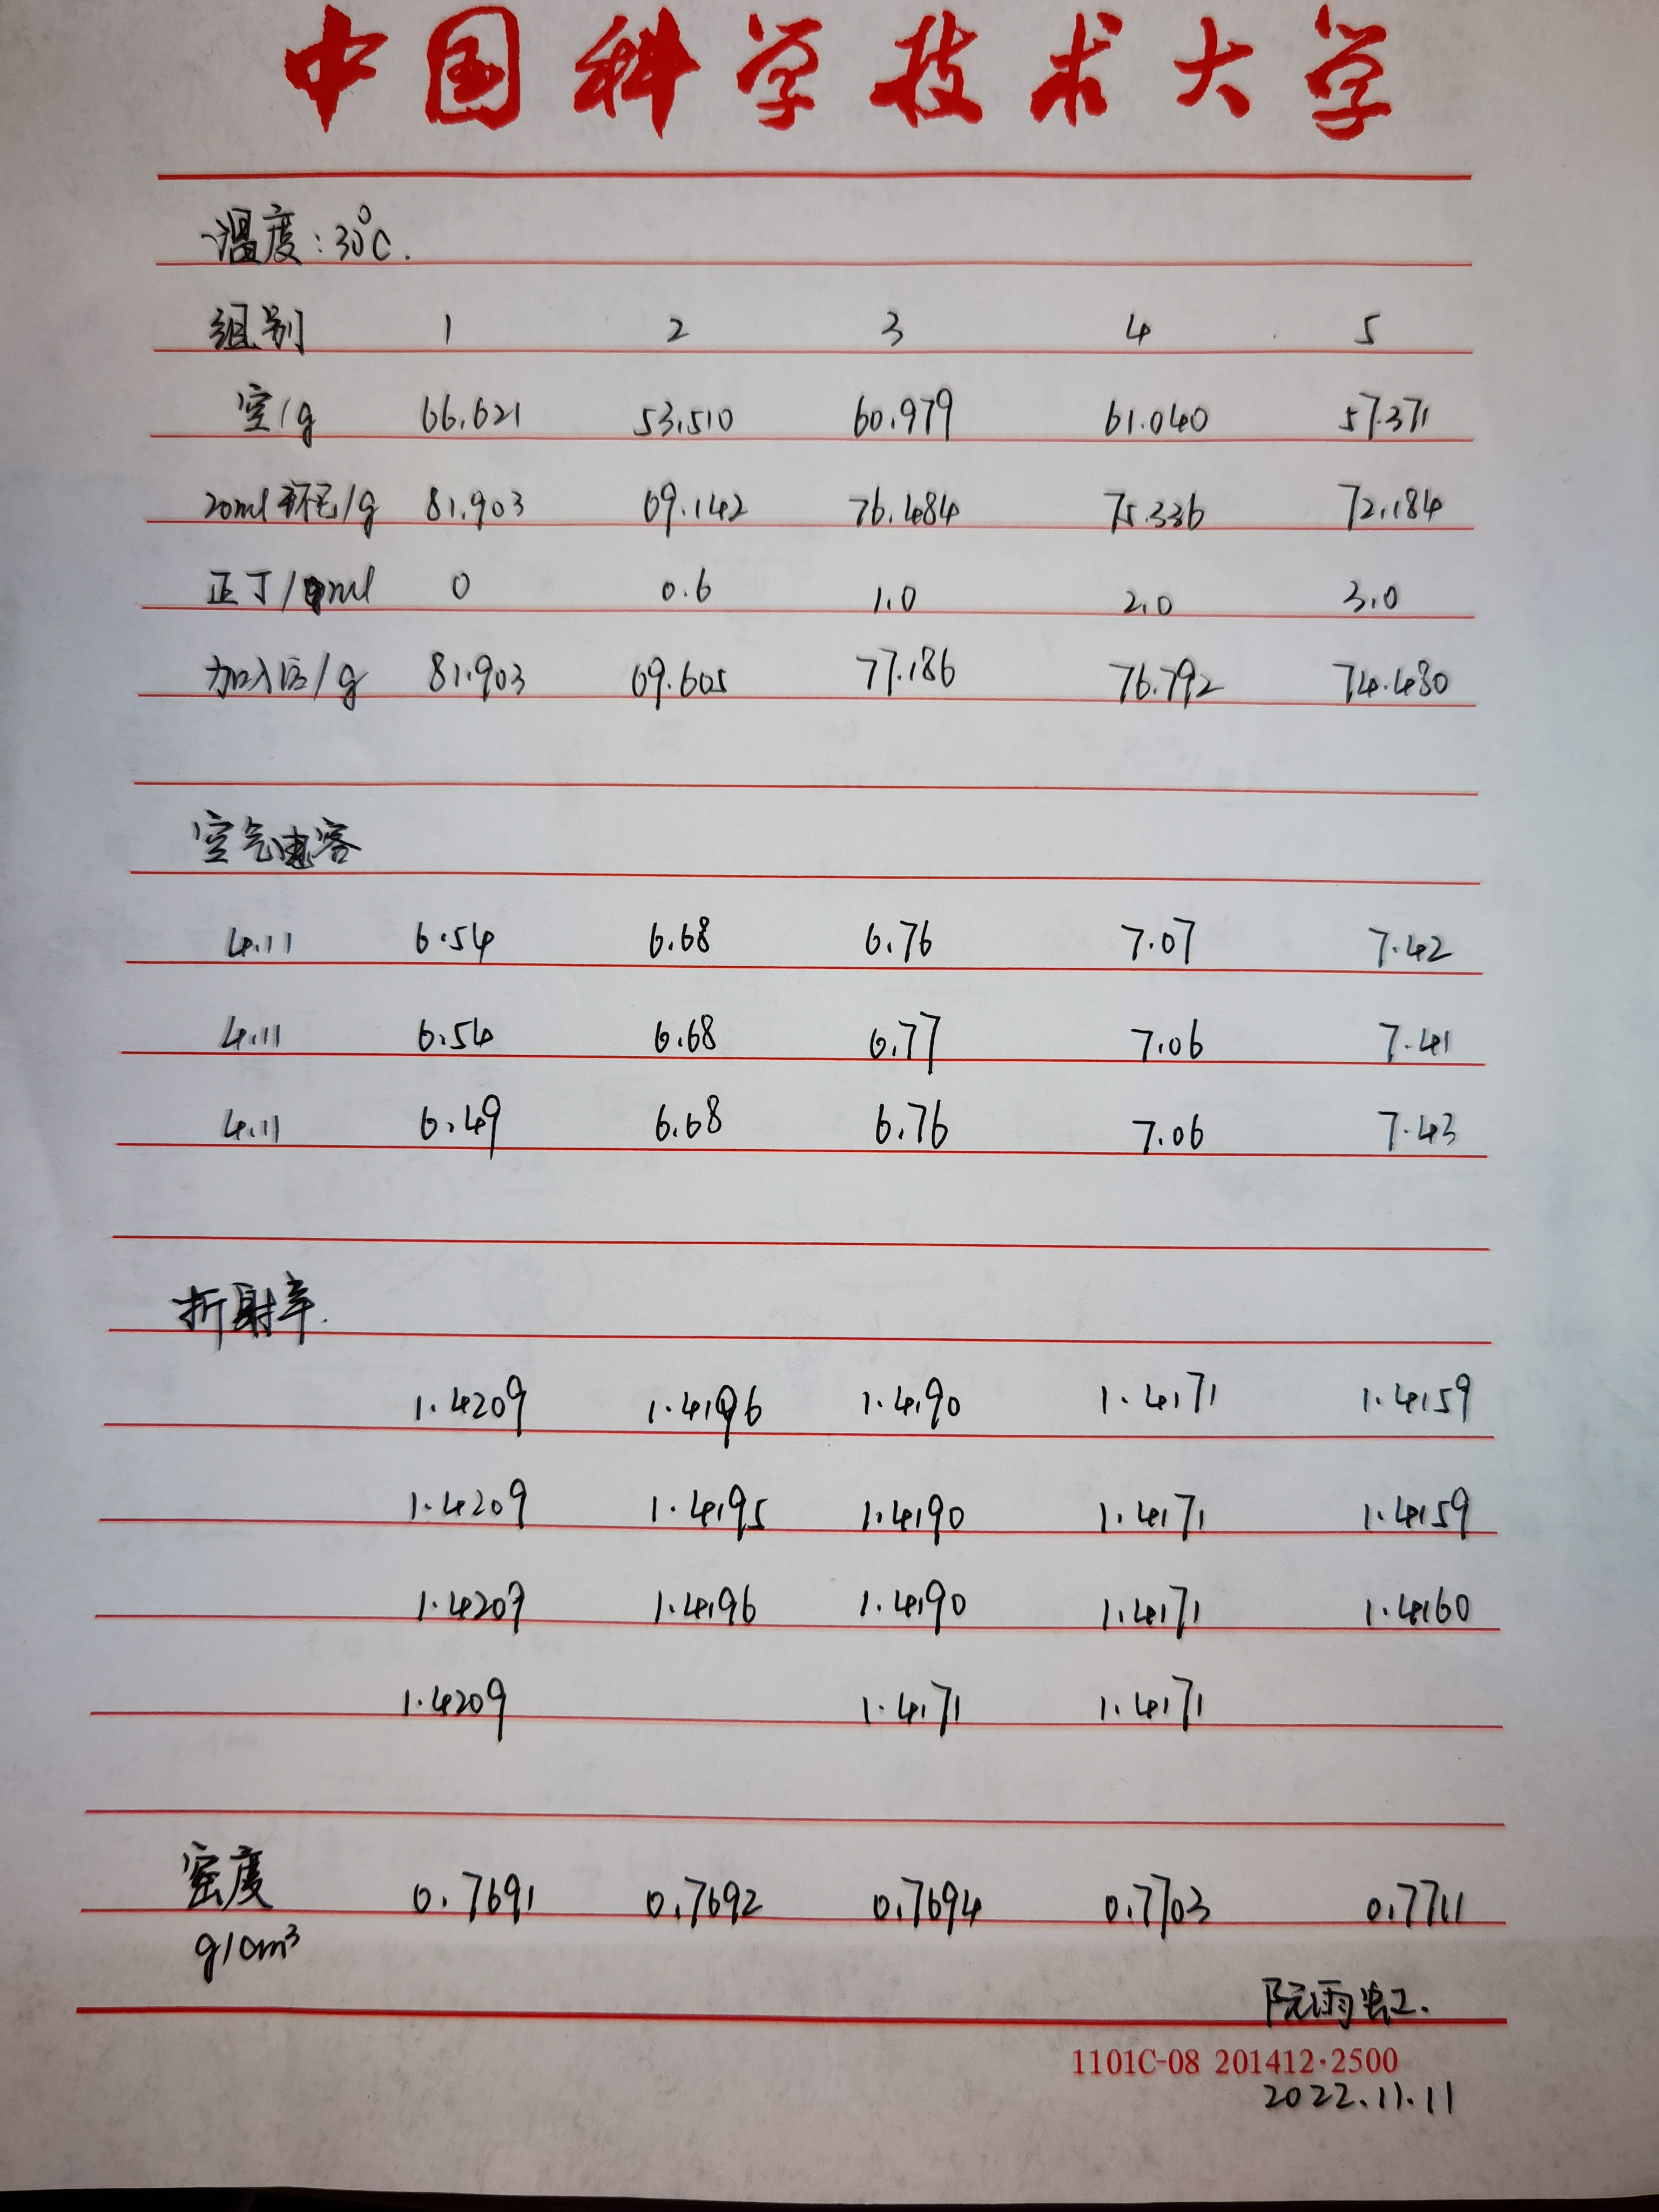
\includegraphics[width=1\textwidth]{data.jpg}
    \caption{原始数据记录}
    \label{fig:data}
\end{figure}


\end{document}
